%%%%%%%%%%%%%%%%%%%%%%%%%%%%%%%%%%%%%%%%%%%%%%
%                insertmeeting
% 1) Title (something creative & funny?)
% 2) Date (MM/DD/YYYY)
% 3) Location (ex. Hagerty High School)
% 4) People/Committees Present 
% 5) Picture 
% 6) Start Time & Stop Time (ex. 12:30AM to 4:30PM)
%%%%%%%%%%%%%%%%%%%%%%%%%%%%%%%%%%%%%%%%%%%%%%
\insertmeeting 
	{Intake Innovations} 
	{10/30/21}
	{Hagerty High School}
	{Nathan, Ritam}
	{Images/RobotPics/robot.jpg}
	{2:30 - 4:30}
	
\hhscommittee{Hardware}
\noindent\hfil\rule{\textwidth}{.4pt}\hfil
\subsubsection*{Goals}
\begin{itemize}
    \item brainstorm intake ideas
    \item design intake to fit with new arm 

\end{itemize} 

\noindent\hfil\rule{\textwidth}{.4pt}\hfil

\subsubsection*{Accomplishments}
As we’ve been doing driver practice with our tank drive robot, we have noticed that the somewhat small size of our intake is one of the greatest hindrances. Although we could simply widen it, the one-block limit means that having an intake large enough to pick up multiple blocks could cause us penalties, especially in a competition when we are moving as quickly as possible and not driving as carefully. While considering this issue, we came up with a design idea that may be able to be wider without increasing the risk of picking up more than one block. This design would put two grabbers right next to each other that would be controlled independently by 2 servos. This would allow us to drive into the warehouse, lining up with a couple blocks. Then, the operator could lower whichever of the two fingers was in a better position to grip a block or ball, leaving the other finger up. Once one finger is down, the driver would back up leaving all of the elements in the warehouse except for the one element that was gripped initially, breaking no rules, but eliminating the need for fine alignment. To better convey this somewhat confusing idea, we created a sketch showing our current design, the too wide design, and our solution (figure 1). 
With this idea roughed out, we started CADing this new intake. Basing this intake on the arm we designed at the last meeting, we quickly realized that many of the arm’s slide joints would need to be modified to hold parts of the intake. The first change we made was editing the slide joint to screw onto the bottom of an intake plate. 
With the basic attachment part made, we created a new part studio and designed the double wide intake. Part of the way through the process, we realized that although it was an odd idea, we may even be able to expand the intake to have 3 grabbers instead of 2. Although we liked the out of the box thinking of this idea, we decided that, at least for now, a triple intake would be too unruly to be effective. Wanting to keep this option possible though, we created the part studio with a variable that allows us to add grabbers, automatically resizing the entire intake to work with as many grabbers as we want. Our new intake design resembles the current one, but we designed more robust, 3d printable fingers that are detached from a servo mount. To reduce weight at the end of the arm, we wanted to move the servo farther up the arm then connect it to the grabber with some wire, allowing the grabbers to be moved by the servos almost like a marionette puppet. To make this idea work with our extendable intake, the servos will have to move with the end of the arm, extending and retracting with the rest of the intake. Because of this, we modified another pair of the arm’s slide joints so that they can hold a laser cut plate that will support our servos and servo mounts. After making all of these parts, we added them into the arm assembly to ensure that everything fit together right.

 

\begin{figure}[ht]
\centering
\begin{minipage}[b]{.48\textwidth}
  \centering
  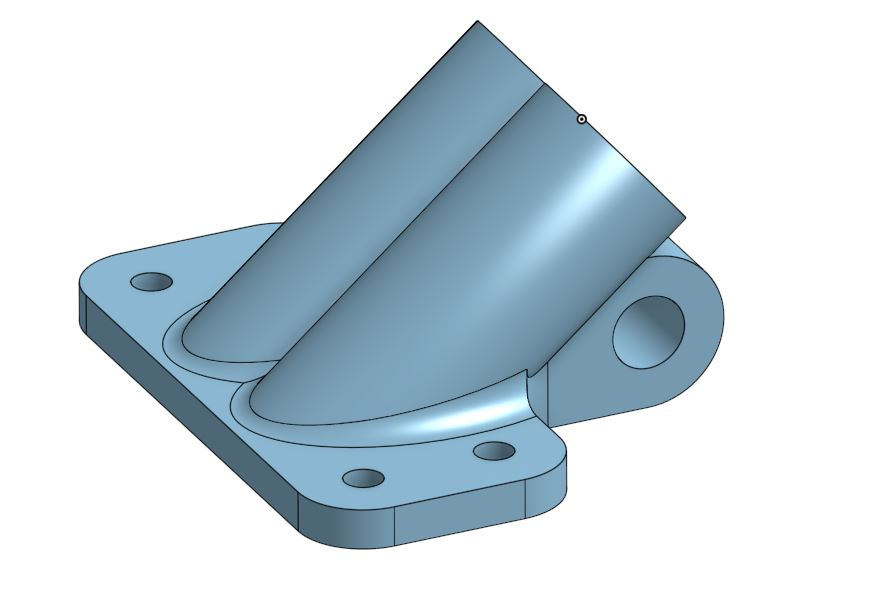
\includegraphics[width=0.95\textwidth]{Meetings/October/10-30-21/10-30-21_CAD_Figure2 - Nathan Forrer.JPG}
  \caption{The new slide joint.}
  \label{fig:pic1}
\end{minipage}%
\hfill%
\begin{minipage}[b]{.48\textwidth}
  \centering
  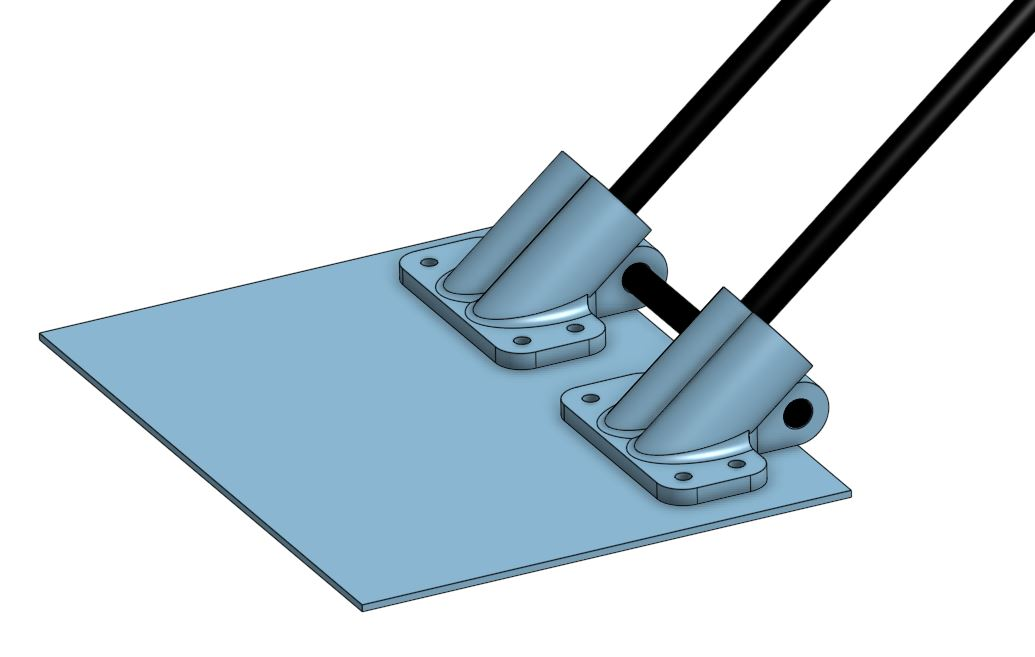
\includegraphics[width=0.95\textwidth]{Meetings/October/10-30-21/10-30-21_CAD_Figure3 - Nathan Forrer.JPG}
  \caption{New slide intake}
  \label{fig:pic2}
\end{minipage}
\end{figure}

\begin{figure}[ht]
\centering
\begin{minipage}[b]{.48\textwidth}
  \centering
  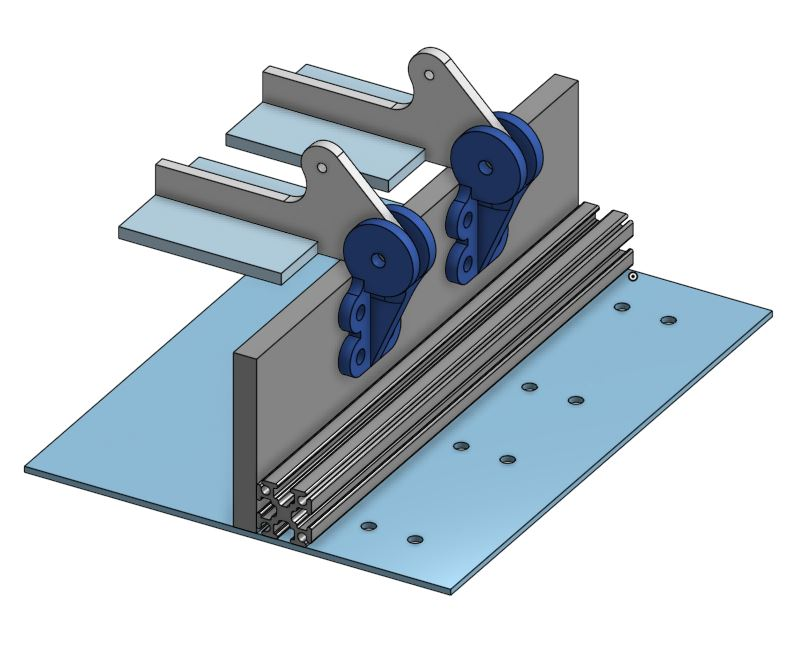
\includegraphics[width=0.95\textwidth]{Meetings/October/10-30-21/10-30-21_CAD_Figure4 - Nathan Forrer.JPG}
  \caption{Intake with movable fingers}
  \label{fig:pic3}
\end{minipage}%
\hfill%
\begin{minipage}[b]{.48\textwidth}
  \centering
  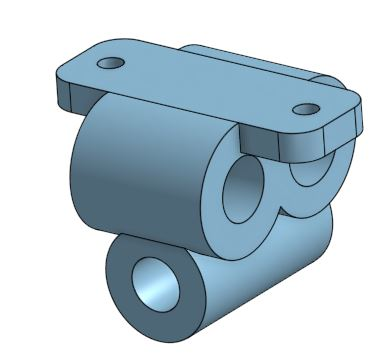
\includegraphics[width=0.95\textwidth]{Meetings/October/10-30-21/10-30-21_CAD_Figure5 - Nathan Forrer.JPG}
  \caption{Servo supports}
  \label{fig:pic4}
\end{minipage}
\end{figure}

\begin{figure}[ht]
\centering
\begin{minipage}[b]{.48\textwidth}
  \centering
  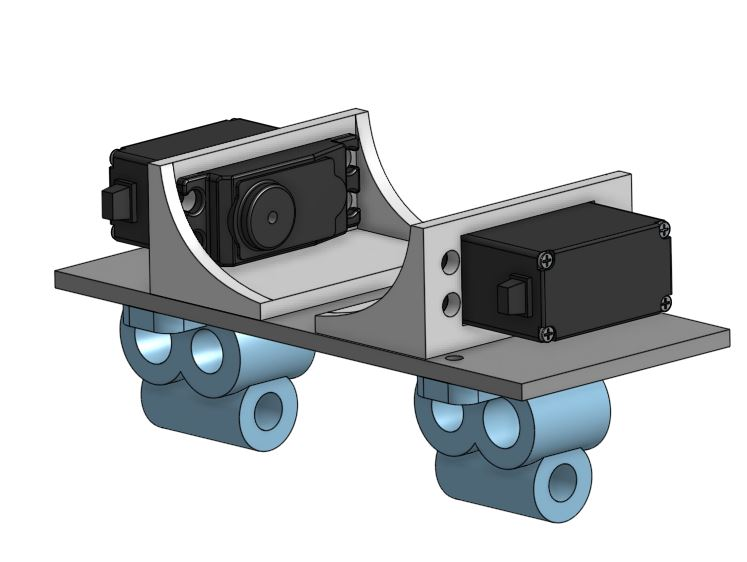
\includegraphics[width=0.95\textwidth]{Meetings/October/10-30-21/10-30-21_CAD_Figure6 - Nathan Forrer.JPG}
  \caption{Servos and servo supports}
  \label{fig:pic5}
\end{minipage}%
\hfill%
\begin{minipage}[b]{.48\textwidth}
  \centering
  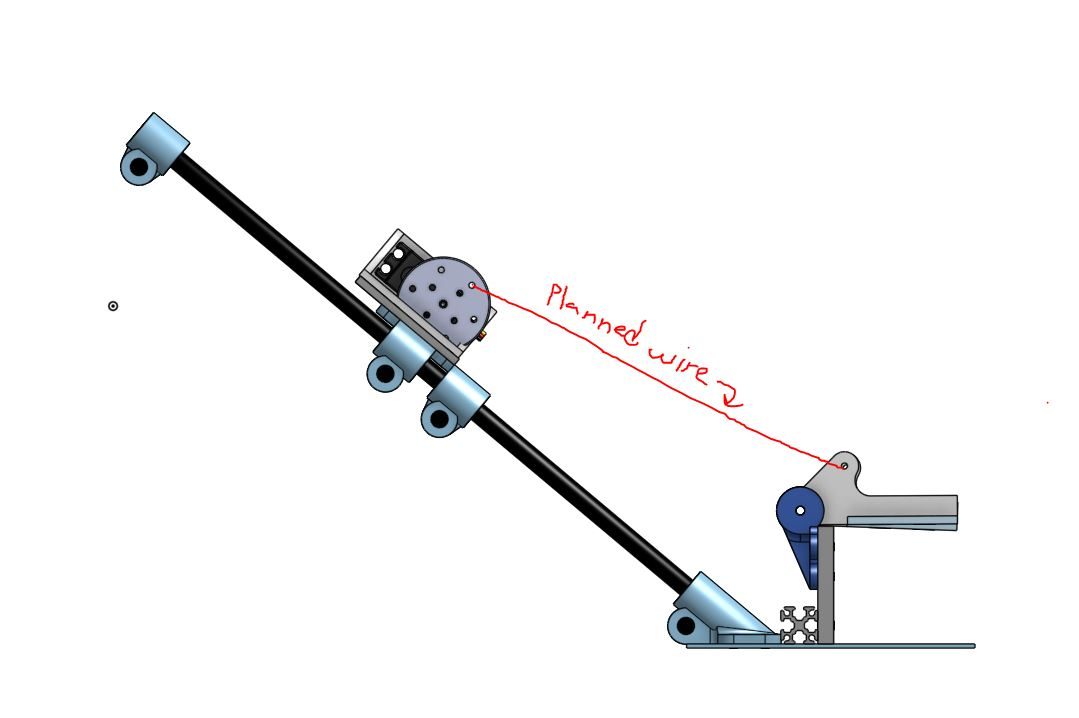
\includegraphics[width=0.95\textwidth]{Meetings/October/10-30-21/10-30-21_CAD_Figure7 - Nathan Forrer.JPG}
  \caption{Side view of arm assembly}
  \label{fig:pic6}
\end{minipage}
\end{figure}

\begin{figure}[htp]
\centering
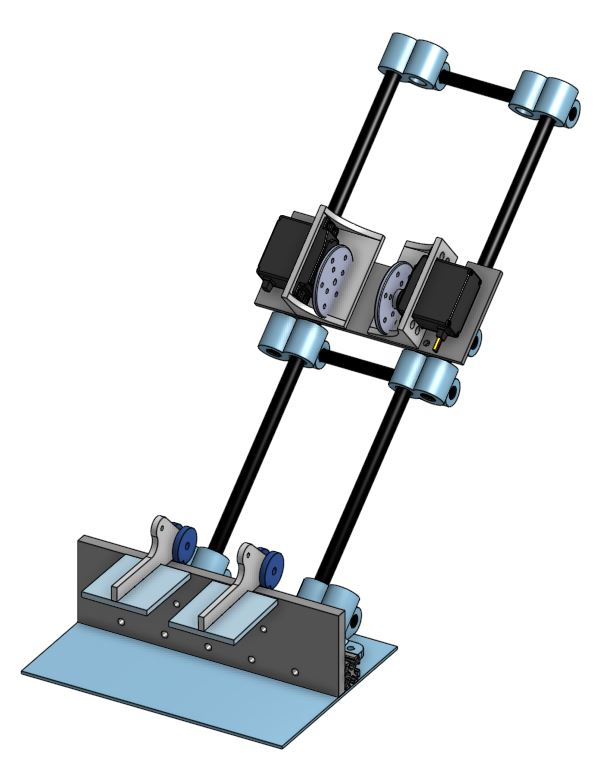
\includegraphics[width=0.95\textwidth, angle=0]{Meetings/October/10-30-21/10-30-21_CAD_Figure8 - Nathan Forrer.JPG}
\caption{Final assembly}
\label{fig:pic7}
\end{figure}

\whatsnext{
\begin{itemize}
    \item Continue working on hardware
    \item Discuss viability of new arm and intake designs

\end{itemize} 
}

